\documentclass[
  % all of the below options are optional and can be left out
  % course name (default: 2IL50 Data Structures)
  course = {{IE579 Game Theory and Multi-Agent Reinforcement Learning}},
  % quartile (default: 3)
  quartile = {{4}},
  % assignment number/name (default: 1)
  assignment = 2,
  % student name (default: Some One)
  name = {{Mohammad Mahdi Rahimi}},
  % student number, NOT S-number (default: 0123456)
  studentnumber = {{20208244}},
  % student email (default: s.one@student.tue.nl)
  email = {{mahi@kaist.ac.kr}},
  % first exercise number (default: 1)
  firstexercise = 1
]{aga-homework}


\usepackage{amssymb,latexsym,amsmath,amsthm}
\usepackage{amsfonts,rawfonts}
\usepackage{thmtools}
\usepackage{systeme}
\usepackage{mathtools}
\usepackage{xcolor}
\usepackage{pgfplots} 
\usepackage{amsmath}
\usepackage{algorithm}
\usepackage[noend]{algpseudocode}
\usepackage{minted}
% \usepackage[margin=1.5in]{geometry}    % For margin alignment


\pgfplotsset{width=10cm,compat=1.9} 
 \usepgfplotslibrary{external}

\tikzexternalize 

\begin{document}

\exercise
\subexercise $x = 1$ Find Pure Nash and SPE
\\\\
Nash Equilibrium :\\
1. \{(R,G),(U)\}\\
2. \{(R,H),(U)\}\\
3. \{(L,G),(D)\}\\
4. \{(L,H),(D)\}\\
\\
Sub-game Perfect Nash Equilibrium :\\
1. \{(R,H),(U)\}


\subexercise Range of x for having (R, U) as unique SPE
\\\\
For $x > 2$ player-1 choose $(L)$, and for $x = 2$ player-1 is indifferent between $(L)$ and $(R)$ in sub-game, so for the range of $x < 2$, $(R, U)$ is the unique SPE.
\\\\
\subexercise  Range of x for having (L) as unique SPE
\\\\
For $x > 2$ player-1 choose $(L)$, and it is the unique SPE.

\exercise
\subexercise Formulate of Game
\\\\
$
N = 4000 \text{(number of Player)}\\\\
A = \{lower, upper\}
a_i: \text{Action Agent i} \\\\
A_{-i}: \text{Action Agents other than i} \\\\
$
\[
U_{x} = 
     \begin{cases}
      {\frac{X}{100}} + 45 &\quad\text {if Choose Upper} \\
      45 + {4000 - x \over 100} &\quad\text{otherwise}\\ 
     \end{cases}
\]

\subexercise Proof (X = 2000) is the Only Nash Equilibrium \\\\
Nash Happen when equal people choose upper and lower road. X = 2000.\\
We show in X = 2000 state, neither upper road agents nor lower road agents wish to change their decision.\\
In state X = 2000 cost of road for all agents equals to 65 minutes any agent who changes the road will increases it's own cost by 0.01 minutes so it's not better score and nothing will change.
\begin{center}
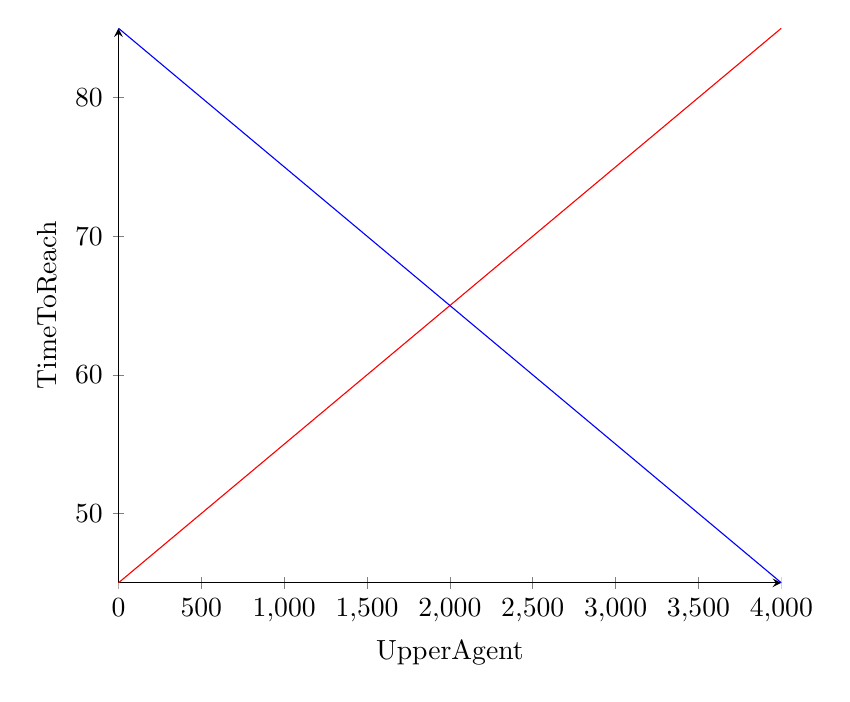
\begin{tikzpicture}
\begin{axis}[
    axis lines = left,
    xlabel = UpperAgent,
    ylabel = TimeToReach,
]
%Below the red parabola is defined
\addplot [
    domain=0:4000, 
    samples=100, 
    color=red,
]
{x/100 + 45};
\addplot [
    domain=0:4000, 
    samples=100, 
    color=blue,
]
{85 - x/100};

\end{axis}
\end{tikzpicture}
\end{center}

Red is upper agents and blue is lower agents.\\
The Only Point that two Best-Response meet as on (2000, 2000).

\subexercise
\[
U_{x} = 
     \begin{cases}
      [1].\ \ {x \over 100} + 45 &\quad\text {if x Agent choose Upper}; X \le 4000 \\
      [2].\ \  40 + {k\over 100} &\quad\text{if k Agent from X choose C-D}; K \le X\\
      [3].\ \  45 + {4000 - x + k \over 100} &\quad\text{otherwise}\\ 
     \end{cases}
\]

\begin{equation} \label{eq1}
\begin{split}
K \le X & \Rightarrow  40 + {k\over 100} < {x \over 100} + 45 \Rightarrow [2] < [1] \\
& \Rightarrow \text{Every Agent In Upper Road can decrease the cost by choosing the C-D,}\\ 
K = X & \Rightarrow 45 + {4000 - x + k \over 1000} = 85 > 40 + {k \over 100} \\
& \Rightarrow \text{Every Agent In Lower Road can decrease the cost by choosing the C-D,}\\
& \Rightarrow \text{Eventually All agent choose C-D road and X = K = 4000}
\end{split}
\end{equation}
The Nash happen when all agents take A-C-D-B road and cost is 80.\\
Surprisingly adding a new road with cost 0 moved Nash from 65 to 80.

\exercise
\subexercise 1. $(B, R, F) \rightarrow (0, 0, 0)$

\subexercise $Max(Min(U_1)) \Rightarrow Max([0, -1]) \Rightarrow [0]$

\subexercise
\begin{center}
\begin{tabular}{ |c|c|c|c| } 
\hline 
 & L & R \\
\hline
\multirow T & 4.4, 4.4 & 1.4, 5.4 \\ 
B & 1.4, 5.4 & 2.4, 2.4 \\ 
\hline
\end{tabular}
\end{center}

\subexercise 1. $(B, R) \rightarrow (2.4, 2.4)$

\exercise
\subexercise Find Nash Equilibrium
\\\\
$
n: \text{Number of Player}\\\\
q_i: \text{Quantity of produce from i-th Firm}\\\\
Q: \text{Action for all Firms} \\\\
Q^{-i}: \text{Action Firms without i-th} \\\\
$
Finding Best Response for i-th Agent by assuming fix action for the rest:\\
\begin{equation} \label{eq1}
\begin{split}
U_i(q_1, ..., q_n) & = U_i(q_i) = \begin{cases}
    (a-Q^{-i}+q_i)q_i - cq_i &\quad\text{if } q_i \le a - Q^{-i} \\
    -cq_i &\quad\text{if } q_i > a - Q^{-i}
\end{cases}
\end{split}
\end{equation}\\
\begin{equation} \label{eq1}
\begin{split}
K = a - Q^{-1} - c
\end{split}
\end{equation}\\
\begin{equation} \label{eq1}
\begin{split}
BR_i(q_i) = argmax(U_i(q_i)) & = \begin{cases}
    argmax(q_i(K - q_i)) &\quad\text{if } q_i \le K + c\\
    argmax(-cq_i) &\quad\text{if } q_i > K + c
\end{cases}\\
& = \begin{cases}
    K \over 2 &\quad\text{if } q_i \le K + c\\
    0 &\quad\text{if } q_i > K + c
\end{cases}
\end{split}
\end{equation}

Assume we are in situation $q_i > K + c$ and everyone will follow BR and set quantity to 0 then we have:

\begin{equation} \label{eq1}
\begin{split}
0 & > K + c \\
0 & > a - Q^{-1} - c + c\\
0 & > a
\end{split}
\end{equation}
It means when '$a$' is less than zero, all firms should stop producing.

Now, Assume we are in situation $q_i \le K + c$ and everyone will follow BR and set quantity to $K \over 2$ then we have:

\begin{equation} \label{eq1}
\begin{split}
Q & = n({K \over 2}) \\
K & = a - Q^{-i} - c\\
K & = a - (n - 1)({K \over 2}) - c\\
(n+1)K & = 2(a - c)\\
K & = {2(a - c) \over (n + 1)}\\
\end{split}
\end{equation}

This is hold when $q_i \le K + c$ it means:
\begin{equation} \label{eq1}
\begin{split}
{K \over 2} & \le K + c\\
0 & \le {K \over 2} + c\\
0 & \le {(a - c) \over (n + 1)} + c
\end{split}
\end{equation}
It means this Best-Response hold when '$c$' is not negative.\\
In a reasonable world both 'a' and 'c' are not negative.\\
Final Price if Firms use BR follow this equation: $P = {K \over 2} = {a - c \over n + 1}$\\

\subexercise Change in Price by adding new Firm\\

Price follow this equation: $P = {a - c \over n + 1}$, It is plotted by assuming 'a - c' equals to 100, for n moving between 0 to 100.

\begin{center}
\begin{tikzpicture}
\begin{axis}[
    axis lines = left,
    xlabel = Number of Firms,
    ylabel = \text{With A-C = 100},
]
%Below the red parabola is defined
\addplot [
    domain=0:100, 
    samples=100, 
    color=red,
]
{100 / (x + 1)};
\end{axis}
\end{tikzpicture}
\end{center}

\exercise
\subexercise Pure Nash and Payoffs
\\
\begin{equation} \label{eq1}
\begin{split}
(B, L) & \rightarrow (8, 2)\\
(T, R) & \rightarrow (2, 8)
\end{split}
\end{equation}

\subexercise Mixed Nash and Payoffs
\begin{equation} \label{eq1}
\begin{split}
({2 \over 3}B + {1 \over 3} T, {2 \over 3}R + {1 \over 3}L)
\end{split}
\end{equation}
\begin{equation} \label{eq1}
\begin{split}
{4 \over 9}(B,R) + {2 \over 9}(B, L) + {2 \over 9}(T, R) + {1 \over 9}(T, L) = ({44 \over 9}, {44 \over 9})
\end{split}
\end{equation}

\subexercise Correlated Equilibrium and Inequalities
\\\\
General Inequalities:\\ 
\begin{equation} \label{eq1}
\begin{split}
\sum{P(R = a | R_i  = a_i) u_i(a_i, a_{-i}}) \ge \sum{P(R = a | R_i  \neq a_i) u_i({a^\prime}_i, a_{-i}})
\end{split}
\end{equation}
\\
Correlated answer set are below:\\ 
\begin{equation}
    \begin{split}
    C \Rightarrow \begin{cases}
    P_1 \Rightarrow 
     \begin{cases}
            T: P(R = L | R_1  = T) u_1(L, T) + P(R = R | R_1  = T) u_1(R, T) \ge\\
            P(R = L | R_1 = B) u_1(L, B) + P(R = R | R_1  = B) u_1(R, B)\\
            B: P(R = L | R_1  = B) u_1(L, B) + P(R = R | R_1  = B) u_1(R, B) \ge\\
            P(R = L | R_1 = T) u_1(L, T) + P(R = R | R_1  = T) u_1(R, T)\\
     \end{cases}\\
    P_2 \Rightarrow 
     \begin{cases}
            L: P(R = T | R_2  = L) u_2(T, L) + P(R = L | R_1  = B) u_2(L, B) \ge\\
            P(R = R | R_2 = T) u_2(R, T) + P(R = R | R_2  = B) u_2(R, B)\\
            R: P(R = T | R_2  = R) u_2(T, R) + P(R = R | R_1  = B) u_2(R, B) \ge\\
            P(R = L | R_2 = T) u_2(L, T) + P(R = L | R_2  = B) u_2(L, B)\\
     \end{cases}\\
    \end{cases}
    \end{split}
\end{equation}

\begin{equation}
    \begin{split}
    P_{LT}u_1(LT) + P_{RT}u_1(RT) & \ge P_{LB}u_1(LB) + P_{RB}u_1(RB) \\
    P_{LB}u_1(LB) + P_{RB}u_1(RB) & \ge P_{LT}u_1(LT) + P_{RT}u_1(RT) \\
    P_{TL}u_2(LT) + P_{BL}u_2(BL) & \ge P_{TR}u_2(TR) + P_{BR}u_2(BR) \\
    P_{TR}u_2(TR) + P_{BR}u_2(BR) & \ge P_{TL}u_2(LT) + P_{BL}u_2(BL)
    \end{split}
\end{equation}

\begin{equation}
    \begin{split}
    P_{LT}6 + P_{RT}2 & \ge P_{LB}8 + P_{RB}0 \\
    P_{LB}8 + P_{RB}0 & \ge P_{LT}6 + P_{RT}2\\
    P_{TL}6 + P_{BL}2 & \ge P_{TR}8 + P_{BR}0 \\
    P_{TR}8 + P_{BR}0 & \ge P_{TL}6 + P_{BL}2
    \end{split}
\end{equation}

\begin{equation}
    \begin{split}
    6P_{LT} + 2P_{RT} & = 8P_{LB} \\
    6P_{TL} + 2P_{BL} & = 8P_{TR} \\
    P_{TR} + P_{BR} + P_{TL} + P_{BL} & = 1
    \end{split}
\end{equation}
\\
After solving equations
\\
\begin{equation}
    \begin{split}
    P_{LT} = P_{RT} = P_{LB} &= P_c\\
    3P_c + P_{BR}& = 1 \Rightarrow P_{BR} = 1 - 3P_c\\
    u_2(P_c) = u_1(P_c) &= P_c(2 + 8 + 6) = 16P_c, P_c \in [0, 1/3]
    \end{split}
\end{equation}
All values that satisfies above equations is a correlated equilibrium.

\subexercise Correlated Equilibrium with Maximum sum of payoffs
\\
\\
Obviously the maximum sum of payoff happen when $P_c$ equals to ${1 \over 3}$ , which means all $P_{LT} = P_{RT} = P_{LB} = {1 \over 3}$ and  $P_{BR} = 0$

\newpage
\exercise
\subexercise Proof
\\
First we direct proof $\overline{V}(A) = \underline{V}(A)\text{ and  } a_{i^\prime j^\prime }\text{ is Nash }\Rightarrow i^\prime \in i_{sec}\text{, } j^\prime \in j_{sec}$ and then use indirect proof for $\overline{V}(A) = \underline{V}(A)\text{ and  } i^* \in i_{sec}\text{, } j^* \in j_{sec}\Rightarrow a_{i^* j^* }\text{ is Nash}$.
\\
\\
Assume $i^* \in i_{sec}$ and $j^* \in j_{sec}$
\begin{equation}
    \begin{split}
    a_{i^\prime j^\prime} \text{is Nash} & \Rightarrow \begin{cases}
        a_{i^\prime j^\prime} = \min_i{a_{j^\prime}} \Rightarrow a_{i^\prime j^\prime} = a_{i^* j^\prime}\\
        a_{i^\prime j^\prime} = \max_j{a_{i^\prime}} \Rightarrow a_{i^\prime j^\prime} = a_{i^\prime j^*}
    \end{cases}\\
    \overline{V}(A) = \underline{V}(A) & \Rightarrow \max_j{a_{i^* j}} = \min_i{a_{i j^*}} = a_{i^* j^*}\\
    \begin{cases}
        a_{i^* j^*} \ge a_{i^* j^\prime}\\
        a_{i^* j^*} \le a_{i^\prime j^*}
    \end{cases} & \Rightarrow \begin{cases}
        a_{i^* j^*} \ge a_{i^\prime j^\prime}\\
        a_{i^* j^*} \le a_{i^\prime j^\prime}
    \end{cases} \Rightarrow a_{i^*, j^*} =  a_{i^\prime j^\prime}
    \end{split}
\end{equation}

\begin{equation}
    \begin{split}
        a_{i^\prime j^\prime} & = a_{i^*, j^*} \\
        \min_i{a_{i j^\prime}} & = min_i{a_{i j^*}}\\
        \Rightarrow \min_i{a_{i j^\prime}} & \ge \min_i{a_{ij}}\\
        \Rightarrow j\prime & \in j_{sec}
    \end{split}
\end{equation}

\begin{equation}
    \begin{split}
        a_{i^\prime j^\prime} & = a_{i^*, j^*} \\
        \max_j{a_{i\prime i}} & = max_j{a_{i^* j}}\\
        \Rightarrow \max_j{a_{i^\prime j}} & \le \max_j{a_{ij}}\\
        \Rightarrow i\prime & \in i_{sec}
    \end{split}
\end{equation}
\\
\\
For Proving $[\overline{V}(A) = \underline{V}(A)\text{ and  } i^* \in i_{sec}\text{, } j^* \in j_{sec} \Rightarrow a_{i^* j^* }\text{ is Nash}]$, let's assume that there are such $i^*$ and $j^*$ which satisfies player security strategy but are not Nash equilibrium. In this case if a Nash equilibrium exists, we assume in $(i^\prime, j^\prime)$ then $a_{i^\prime j^\prime}$ should be less than $a_{i^*, j^\prime}$ and more than $a_{i^\prime j^*}$, Which leads to $i^*$ and $j^*$ are no longer a security strategies and it contrast with our primary assumptions, so $(i^*, j^*)$ should be a Nash equilibrium.

\subexercise Proof

\begin{equation}
    \begin{split}
        a_{i_1j_1} & \Rightarrow \begin{cases}
        a_{i_1j_1} \le min_i{a_{ij_1}} \Rightarrow a_{i_1j_1} \le a_{i_2j_1}\\
        a_{i_1j_1} \ge max_j{a_{i_1j}} \Rightarrow a_{i_1j_1} \ge a_{i_1j_2}
        \end{cases}\\
        a_{i_2j_2} & \Rightarrow \begin{cases}
        a_{i_2j_2} \le min_i{a_{ij_2}} \Rightarrow a_{i_2j_2} \le a_{i_1j_2}\\
        a_{i_2j_2} \ge max_j{a_{i_2j}} \Rightarrow a_{i_2j_2} \ge a_{i_2j_1}
        \end{cases}
    \end{split}
\end{equation}

\begin{equation}
    \begin{split}
         & a_{i_1j_1} \le  a_{i_2j_1} \le  a_{i_2j_2} \le  a_{i_1j_2} \le  a_{i_1j_1}\\
         \Rightarrow & a_{i_1j_1} =  a_{i_2j_1} =  a_{i_2j_2} =  a_{i_1j_2}\\
         \Rightarrow & \text{Therefore, all four points are Nash equilibrium}
    \end{split}
\end{equation}

\newpage
\exercise

\subexercise Disproof.
It might fall into a loop depending of initial actions and size of the game. (For 2 by 2 it works fine)\\
Example is below table when non of start actions are 1.\\
\begin{center}
\begin{tabular}{ |c|c|c|c| } 
\hline 
 & 0 & 1 & 2 \\
\hline
\multirow 0 & 2 , 0 & 1 , 1 & 0 , 2 \\ 
\hline
1 & 1 , 1 & 3 , 3 & 1 , 1 \\ 
\hline
2 & 0 , 2 & 1 , 1 & 2 , 0 \\ 
\hline
\end{tabular}    
\end{center}

\subexercise New Algorithm.\\\\

Assume we have a two-player normal form game in which players has $n_i$ actions.
We can use dynamic programming approach and split the game of $n_1 * n_2$ to a 4 sub-game of $\lceil {n_1 \over 2} \rceil * \lceil {n_2 \over 2} \rceil$ and after solving each sub-game we might reach a Nash for each of them with two corresponding actions, then we reduce our four answers to a new $2 * 2$ game and find the Nash for $2*2$ with BestResponce-Algorithm which shown in last part.

\begin{minted}{python}
def find_nash_final(G):
    actions = []  # Two corresponding action which leads to Nash
    value = 0.0  # value of the Nash
    # Find Nash by given algorithm using BestResponse
    return actions, value
def find_nash(G):
    n1 = len(G); n2 = len(G[0])
    if n1 < 3 or n2 < 3:
        return find_nash_final(G)
    else:
        half_n1 = floor(n1 / 2); half_n2 = floor(n2 / 2)
        # Create four sub-game
        sub_game = [
            G[:half_n1, :half_n2],
            G[:half_n1, half_n2:],
            G[half_n1:, :half_n2],
            G[half_n1:, half_n2:]
        ]
        # Find Nash of each sub-game
        actions = []; values = []
        for game in sub_game:
            act, val = find_nash(game)
            actions.append(act)
            values.append(val)
        # Create the final game with four state
        final_game = [
            [values[1], values[2]],
            [values[3], values[4]]
        ]
        # Solve the final game and return Nash Equilibrium actions and
        act, val = find_nash_final(final_game)
        return actions[act[0] * 2 + act[1]], val
\end{minted}{python}

\proof Assume a pure Nash Equilibrium exists for this game, so it will remains a Nash in any sub-game of this game which contain that state. This algorithm have two phase of divide and merge, which will be discussed in below.\\\\
(1) In divide phase, after we recursively divide the game to sub-games with size less than 3, we have the opportunity to solve them. In this phase the general pure Nash will surely be selected as Nash of its own sub-game and send to next level. (Definition of pure Nash)
\\\\
(2) In merge phase, we create a new sub-game of with four winner state of child sub-games and the general Nash from previous step will be shown in a new sub-game and continue to winning till reach the final game.
\\\\
Therefore, at the end the general pure Nash will not get lost, and we find it's values and corresponding actions.
\\\\
\textbf{Calculation Time-Complexity}\\
Assume player 1 has $N$ and player 2 has $M$ actions and $N \ge M$.\\\\
Sub Game(Case 1): $T_{nash}(0*0) = 0, T_{nash}(1*1) = 0, T_{nash}(2*2) = 4$\\
Sub Game(Case 2): $T_{nash}(0*N) = 0, T_{nash}(1*N) = N, T_{nash}(2*N) = 2*N$\\
\\
Sub Game Order Worst: $O(SubGame) = O(N)$\\
Sub Game Order Best: $O(SubGame) = constant $\\\\
Divide: $T_{divide}(MN) = 4T_{divede}(MN/4) = 4^{\log_4{MN}}*T_{subgame} = MN*T_{subgame}$\\\\
Total Order Worst: $O(Game) =  O(MN) * O(N) = O(MN^2)$\\
Total Order Best: $O(Game) = O(MN) * constant = O(MN)$\\\\
Total Order $M = N$: $O(Game) = O(N^2) * constant = O(N^2)$\\\\

\end{document}
